\documentclass{article}
\usepackage{tikz}
\usepackage{pgf-umlcd}

\begin{document}

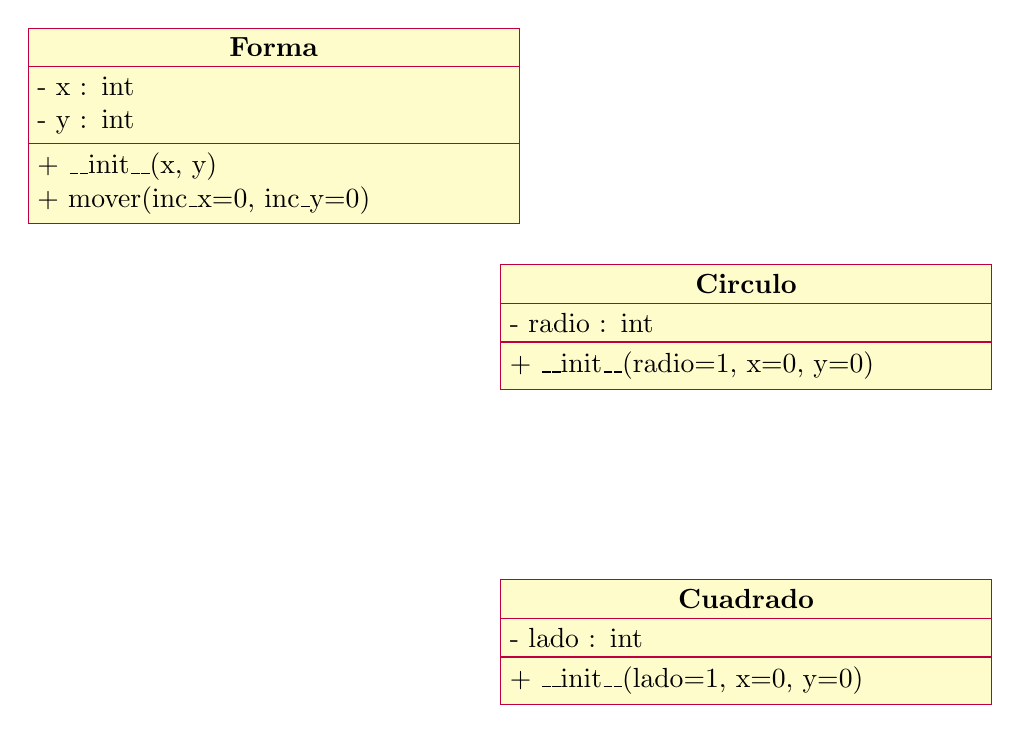
\begin{tikzpicture}

% Clase base
\begin{class}[text width=6cm]{Forma}{0,0}
\attribute{- x : int}
\attribute{- y : int}
\operation{+ \_\_init\_\_(x, y)}
\operation{+ mover(inc\_x=0, inc\_y=0)}
\end{class}

% Subclase Círculo
\begin{class}[text width=6cm]{Circulo}{6,-3}
\attribute{- radio : int}
\operation{+ \_\_init\_\_(radio=1, x=0, y=0)}
\end{class}

% Subclase Cuadrado
\begin{class}[text width=6cm]{Cuadrado}{6,-7}
\attribute{- lado : int}
\operation{+ \_\_init\_\_(lado=1, x=0, y=0)}
\end{class}

% Relaciones de herencia
\inherit{Circulo}{Forma}
\inherit{Cuadrado}{Forma}

\end{tikzpicture}

\end{document}
